\chapter{含风电电力系统脆弱性理论}
\label{cha:theory}

\section{引言}
\label{sec:index3}


\section{含风电电力系统结构脆弱性研究}
\label{sec:powersys}

\subsection{含风电电力系统结构脆弱性}
\label{sec:vulneStuct}
风力发电系统的结构主要指的是除发电机、负荷之外,电能被输送的网络的拓扑。拓扑是整个网络性能的基础,它决定了电能是否能够被安全、有效、可靠的输送到负荷端。但是,受外界环境的干扰、人为干预、不可抗力的影响,拓扑的结构并非一尘不变,其组成元素都有遭到破坏的可能。因此,有必要衡量拓扑的各个组成元素在结构上的重要性,这对于提前加强防范、预先保护有着重要的意义。

本文在前人研究的基础上对结构脆弱性提出了新的定义:电力系统的结构脆弱性是指电力系统因人为或外界不可抗力的影响下,自身组成因素遭到破坏后不能保持系统结构完整的特性。对系统结构完整性贡献的程度高、对拓扑结构关键程度高的组成元素被称为系统结构的脆弱点。因此,对电力系统的结构越重要,影响越大的组成因素的脆弱性越高。

风力发电系统的结构建模有多种,本文分别从复杂网络的角度和互联网网页重要度排序的角度进行研究。前者将电网抽象为一个加权无向图,后者将电网等效为一个有向图。二者出发的角度不同,建模方式不同,但是都从结构上对电网节点的重要性进行了评估。本文对这两种建模方法进行了研究和对比,将各自的模型指标在第四章中进行了融合评估。

\subsection{基于复杂网络的结构脆弱性研究}
\label{sec:network}
复杂网络的基本思想是将一个复杂系统抽象为网络,其中系统中的单个个体被视为网络的节点,而个体之间的联系被视为网络的边,由此建立复杂网络模型。对于含风电电力系统而言,系统中的母线可以被视为节点,而母线之间的电气连接可以被视为边,线路上的阻抗为权重,因此整个系统可以被等效为一个加权无向图。

复杂网络理论中描述网络的特征参数有特征路径长度、节点度和节点度累计分布、聚类系数、介数和介数分布等。

$(1)$特征路径长度$(L)$
特征路径长度定义为所有节点对之间最短距离的均值,其中,$d_{ij}$为连通网络节点$i$和$j$之间一条最短路径所覆盖的变数,$N$为网络中的节点数量。
\begin{equation}
\label{equ:chap3:Index01}
L=\displaystyle\frac{1}{N(N-1)}\sum_{i\neq j}d_{ij}
\end{equation}

$(2)$节点度和节点度累积分布
节点度定义为与该节点相连的所有节点的数量。节点度分布是指网络中出现节点度为$k$的节点个数所占总节点数的比例。

$(3)$聚类系数$(C)$
聚类系数是一个表征邻接点间联系紧密程度的特征参数。假设某个节点i的节点度为$i$,则相邻节点之间的边数最大为$\frac{k_i(k_i-1)}{2}$,假设$k_i$个相邻节点之间有$t_i$条边,则节点$i$的聚类系数定义为:$C_i=\frac{2t_i}{k_i(k_i-1)}$,求平均之后得到聚类系数:
\begin{equation}
\label{equ:chap3:Index02}
L=\displaystyle\frac{1}{N}\sum_{i=1}^{N}C_i
\end{equation}

$(4)$介数和介数分布
网络中的介数定义为假设两个节点间的信息总是沿着节点间最短路径传播的,通过某个节点或边的最短路径次数可以表征该节点或边在信息传播过程中的重要性。最短路径通过该节点或边的次数越多,该节点或边对整个网络的贡献越多,其重要性也越高。其中,$\sigma_{ij}$是指节点$i$、$j$间最短路径的数量,$\sigma_{ij}(v)$是指节点$i$、$j$间最短路径通过节点$v$的数量,$\sigma_{ij}(e)$是指节点$i$、$j$间最短路径通过边$e$的数量。

\begin{equation}
\label{equ:chap3:Index03}
C_B(v)=\sum_{i\neg j \in V}\displaystyle\frac{\sigma_{ij}(v)}{\sigma_{ij}}
\end{equation}
\begin{equation}
\label{equ:chap3:Index04}
C_B(e)=\sum_{i\neg j \in V}\displaystyle\frac{\sigma_{ij}(e)}{\sigma_{ij}}
\end{equation}

其中,介数作为复杂网络的关键参数之一,被用来描述节点或者边在信息、能量传递中的重要程度。介数的概念在电力系统被称为电气介数,它反映了网络节点、支路在整个电能输送过程中的贡献程度。假设一个电网具有$a$个母线节点,$b$条电气连接的边,那么支路$l_{mn}$的电气介数计算公式为:
\begin{equation}
\label{equ:chap3:Index1}
C_{B}(m,n)=\left|\sum_{i\in\mathbf{G},j\in\mathbf{D}}w_{ij}P_{mn}(i,j)\right|
\end{equation}
其中,$G$,$D$分别为发电节点、负荷节点的集合。$P_{mn}(i,j)$是单位有功功率注向发电节点$i$和负荷节点$j$时,支路$l_{mn}$上产生的有功功率。$w_{ij}$是发电节点$i$到负荷节点$j$的节点对间传输电能的权重值,大小为$min(|P_i|,|P_j|)$,分别代表了发电节点$i$在发电节点功率总和的比率和负荷节点$j$在负荷节点功率总和的比率。

电网中节点的分类分为发电节点,负荷节点,中间节点。所有的功率都是从发电节点向负荷节点传输,因此需要对上述公式进行修正。式~(\ref{equ:chap3:Index2})中,$F(k)$指的是与节点$k$相连的所有边的集合,$C_B(k,l)$为对应支路的电气介数。
\begin{equation}\label{equ:chap3:Index2}
C_B(k)= \begin{cases}
        \displaystyle\frac{1}{2}\left(\sum\limits_{l\in\mathbf{F(k)}}{C_B(k,l)}+\sum\limits_{i\in\mathbf{D}}{w_{ki}}\right), &  k\in\mathbf{G} \\
        \displaystyle\frac{1}{2}\left(\sum\limits_{l\in\mathbf{F(k)}}{C_B(k,l)}+\sum\limits_{i\in\mathbf{G}}{w_{ik}}\right), &  k\in\mathbf{D} \\
        \displaystyle\frac{1}{2}\left(\sum\limits_{l\in\mathbf{F(k)}}{C_B(k,l)}\right) & k\not\in\mathbf{G},k\not\in\mathbf{D} \\
      \end{cases}
\end{equation}

电气介数不局限于能量、信息沿着网络的最短路径传播,更体现了电能在整个网络支路的分布情况。同时,电气介数还分别考虑了发电节点和负荷节点的变化影响,改变他们的容量,网络各节点的重要性也会发生变化,因此,电气介数更符合实际电网的变化情况。

\subsection{基于$PageRank$的结构脆弱性研究}
\label{sec:pagerank}
$PageRank$最早是被用来作为互联网网页结构的模型,并且对所有网页的重要度进行量化评估的一种算法。在众多计算互联网网页的相关性的算法中,$PageRank$是名气最大,且最早被谷歌浏览器采用的。$PageRank$的基本思想是一个网页的重要性依赖于所有链接向它的其他网页。比如,网页$i$有链接指向网页$j$,如果有很多其他网页有链接指向网页$j$,那么我们认为,网页$j$是非常重要的。另一方面,若只有一个网页有链接指向网页$j$,但是这个网页是一个权威性很高的网址,如谷歌,百度等网页,我们认为网页$j$也非常重要,因为由受欢迎、权威的网页指向它,这份重要性将会传递下来。

电网中,每条支路上的潮流是有确定的方向的,所以可以被视为一个有向图。其中,每个母线节点被视为一个网页,母线节点之间的电气连接被视为网页中的超链接,根据电流的方向决定超链接的方向。互联网与电网的$PageRank$的拓扑模型比较如表~\ref{tab:PRComparision}。根据$PageRank$模型中,网页的超链接可以传递重要性的思想,假设$A$网页拥有~3~个出链,它会分别传递给$B$、$C$、$D$三个网页各自$\frac{1}{3}$的重要性。根据重要性传递规则,可以得到连接$P$。
\begin{table}[htb]
  \centering
  \caption{互联网与电网的$PageRank$拓扑模型比较}
  \label{tab:PRComparision}
    \begin{tabular}{C{4.5cm}C{4.5cm}C{4cm}}
      \toprule
      互联网 & 电网 & $PageRank$拓扑 \\
      \midrule
      网页 & 母线 & 节点\\
      超链接 & 输电支路 & 有向边\\
      指向该网页的网页数目 & 母线进线数目 & 入度\\
      该网页指向的网页数目 & 母线出线数目 & 出度\\
      \bottomrule
    \end{tabular}
\end{table}

$PageRank$算法的具体步骤为:$(1)$假定初始服从均匀分布,即每个网页的重要性都是相同的,即对于一个一共有$n$个节点的系统而言,赋予每个网页相同的$PR$值,一般都为1。$(2)$迭代计算,由于每个超链接的存在都会增加对应网页的$PR$值,所以通过考虑潮流连接情况对各个母线节点的$PR$值进行迭代更新,具体公式如~(\ref{equ:chap3:Index3})。$(3)$最后,经过若干次的迭代后,各个母线节点的$PR$值会趋于一个稳定的值。
\begin{equation}
\label{equ:chap3:Index3}
PR(p_i)=\frac{1-q}{N}+q\sum\limits_{p_j\in\mathbf{M_{p_i}}}{\frac{PR(p_j)}{L(p_j)}}
\end{equation}

式~(\ref{equ:chap3:Index3})中,$p_i$是被计算的节点,$M_{p_i}$是节点$p_i$的入链节点集合,$L(p_j)$是节点$p_j$的出链数目,$N$是节点总数目。$q$为阻尼系数,一般取~0.85~,引入该参数是为了解决出链为零的节点在模型计算中带来的问题,代表了当前的母线节点没有遭到破坏正常运行的概率。$1-q$则代表了节点遭到意外破坏退出运行的概率。$PR$值代表了节点在网络中的重要程度,$PR$值越高,节点越重要。

\section{含风电电力系统状态脆弱性研究}
\label{sec:status}
对于含风电电力系统而言,外界环境的变化会导致系统有多种运行状态,其中环境的变化主要指的是是风速的变化和负荷需求的变化。在这种情况下,系统的状态决定了系统是否能够正常运行下去。因此,研究系统的状态脆弱性对评估系统是否安全运行具有重要的意义。

\subsection{含风电电力系统的状态脆弱性}
\label{sec:vulneStaus}
在电力系统状态的研究中,潮流计算扮演了重要的角色,系统的每一种运行状态对应了一种潮流分布。在变化的潮流参数中,主要关注的参数是电压幅值,电压相角,有功功率和无功功率。能够正常运行的状态通常都是满足以下两点约束:

$(1)$负荷供电约束:系统的所有节点都应满足各自的功率方程,即各节点的有功负荷与无功负荷应保持平衡。
$(2)$运行参数约束:系统的所有节点的电压、功率都应在一定的范围约束内,如节点电压不能越线,支路功率不能太大等。

根据系统的运行状态可以将系统划分出几个区域,如图\ref{fig:sysDomain}。其中,正常域表示系统可以正常运行,脆弱域表示系统可以运行,但运行参数超出了可接受范围,有可能往坏的趋势发展。这两个区域都是可运行域,即系统可以运行的区域。而不可运行域表示系统已经潮流不收敛,负荷不再守恒的故障状态。
\begin{figure}[H] % use float package if you want it here
  \centering
  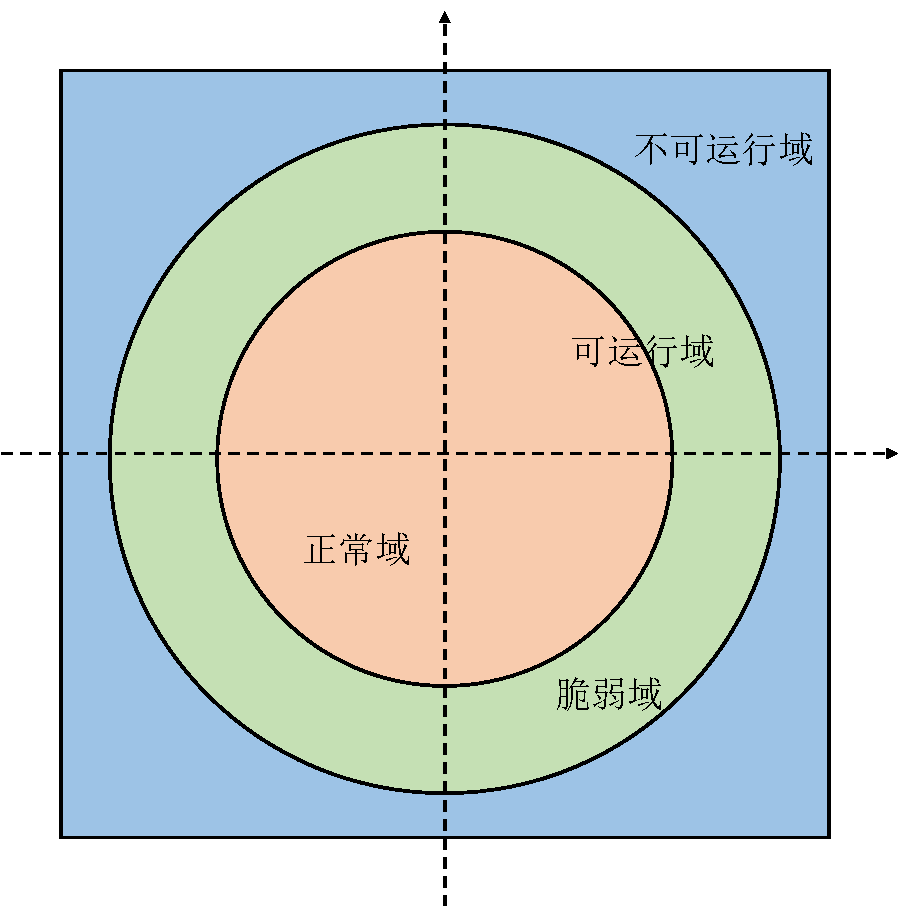
\includegraphics[height=9.5cm]{sysDomain.pdf}
  \caption{电力系统运行状态图}
  \label{fig:sysDomain}
\end{figure}

本文在前人研究的基础上对状态脆弱性提出了新的定义:电力系统的状态脆弱性是指外界环境的变化(如风速、负荷)导致系统无法正常运行,向坏的方向发展,无法恢复正常运行的一种趋势。对外界环境的变化敏感且容易往坏的方向发展的环节被称为脆弱环节。因此,环境变化的影响越大,对系统的运行状态影响越大的环节越脆弱。

补

\subsection{基于的状态脆弱性研究}
\label{sec:dynamic}

\subsection{基于概率潮流的状态脆弱性研究}
\label{sec:static}


\section{风力发电系统脆弱性描述}
\label{sec:defina}

\section{本章小结}
\label{sec:sum3} 